\documentclass[9pts]{article}
\usepackage[utf8]{inputenc}
\usepackage[top=2.5cm, bottom=2.5cm, left=1.5cm, right=1.5cm]{geometry}

\usepackage{listings}
\usepackage{color}
\usepackage{graphicx}
\usepackage{caption}

\definecolor{mygreen}{rgb}{0,0.6,0}
\definecolor{mygray}{rgb}{0.5,0.5,0.5}
\definecolor{mymauve}{rgb}{0.58,0,0.82}

\lstset{
  backgroundcolor=\color{white},   % choose the background color; you must add \usepackage{color} or \usepackage{xcolor}; should come as last argument
  basicstyle=\footnotesize,        % the size of the fonts that are used for the code
  breakatwhitespace=false,         % sets if automatic breaks should only happen at whitespace
  breaklines=true,                 % sets automatic line breaking
  captionpos=b,                    % sets the caption-position to bottom
  commentstyle=\color{mygreen},    % comment style
  deletekeywords={...},            % if you want to delete keywords from the given language
  escapeinside={\%*}{*)},          % if you want to add LaTeX within your code
  extendedchars=true,              % lets you use non-ASCII characters; for 8-bits encodings only, does not work with UTF-8
  frame=single,	                   % adds a frame around the code
  keepspaces=true,                 % keeps spaces in text, useful for keeping indentation of code (possibly needs columns=flexible)
  keywordstyle=\color{blue},       % keyword style
  language=Octave,                 % the language of the code
  morekeywords={*,...},            % if you want to add more keywords to the set
  numbers=left,                    % where to put the line-numbers; possible values are (none, left, right)
  numbersep=5pt,                   % how far the line-numbers are from the code
  numberstyle=\tiny\color{mygray}, % the style that is used for the line-numbers
  rulecolor=\color{black},         % if not set, the frame-color may be changed on line-breaks within not-black text (e.g. comments (green here))
  showspaces=false,                % show spaces everywhere adding particular underscores; it overrides 'showstringspaces'
  showstringspaces=false,          % underline spaces within strings only
  showtabs=false,                  % show tabs within strings adding particular underscores
  stepnumber=2,                    % the step between two line-numbers. If it's 1, each line will be numbered
  stringstyle=\color{mymauve},     % string literal style
  tabsize=2,	                   % sets default tabsize to 2 spaces
  title=\lstname                   % show the filename of files included with \lstinputlisting; also try caption instead of title
}

\title{[4AI02] Projet de C++ Avancé: Algorithme de Dijkstra}
\author{
  Géhère, Kévin\\
  \texttt{kevin.gehere@sorbonne-universite.fr}
  \and
  Fraillon, Vincent\\
  \texttt{vincent.fraillon-maison@sorbonne-universite.fr}
}

\begin{document}
\maketitle

\section{Temps et notation}

Trois séances de 4H chacune sont mis à disposition pour réaliser ce projet.
Les étapes à réaliser sont suggérées dans la feuille de route au chapitre \ref{sec::feuille}. Le rythme n'est pas imposé étant donné que la soumission du projet est possible à tout moment lors de la période du projet.
Des programmes de test sont fournis afin d'évaluer le code et d'estimer le niveau d'accomplissement du projet.\\

Notation :
\begin{itemize}
\item Instantiation des classes ($+$3pts $=>$ 3$/$20);
\item Implémentation de read\_stations ($+$3pts $=>$ 6$/$20);
\item Implémentation de read\_connections ($+$3pts $=>$ 9$/$20);
\item Génération du graphe ($+$4pts $=>$ 13$/$20);
\item Estimation du meilleur chemin et affichage ($+$7pts $=>$ 20$/$20);
\item Amélioration ($+$5pts $=>$ 25$/$20);
\item Bonus : Proposition d'un nom et d'un logo pour votre start-up ($+$1pt)
\item Chaque critère de la charte d'écriture (Voir Chapitre \ref{sec::charte}) fera perdre 1,5 point ($-1,5$pts).\\
\end{itemize}

Tout point au dessus de 20 sera utilisé comme bonus pour les 4 premiers TPs.\\

Date limite du rendu du code : \textbf{Vendredi 13 avril 2018, 20h00}. Chaque minute de retard fera perdre un point sur la note du projet. Un rendu contient le code nécéssaire pour pouvoir compiler le projet en une seule commande, de même pour l'éxécution. Ces commandes peuvent être définies par example dans un fichier \emph{lisez-moi}). \\

La soumission du projet se fera sur l'espace Moodle dédié. La soumission multiple est possible, la dernière soumission écrasant les précédentes.


\section{Introduction}
Vous êtes membre d'une start-up qui veut se lancer sur le marché de la vente de données de trafic.
Pour ce faire il faut implémenter un algorithme capable de planifier des temps de parcours au moyen d'une heuristique fixe, ou dynamique.
Une base de données réaliste et fiable pour le tester est requis pour établir la validité de son implémentation et du cadre dans lequel va naître le projet.
L'algorithme de Dijkstra et la base de données libre de la RATP sont des choix logiques car robustes.
Après concertation, un contrat est écrit pour juger des fonctionnalités minimums ne fréinant pas l'évolutivité de la solution.
L'équipe a reçu le cahier des charges des commerciaux qui demande les fonctionnalités minimum du projet que les ingénieurs ont traduit en contrat de programmation. La tâche est de réaliser un programme correct respectant la structure imposée. Une recherche sera nécéssaire afin de maitriser l'algorithme de Dijkstra, afin de pouvoir l'implémenter.

\subsection{Une résolution du problème du plus court chemin}
Le but de ce projet est de faire une application qui dit quel est le trajet le plus court entre deux stations du métro Parisien.

\begin{figure}[h]
   \centering
   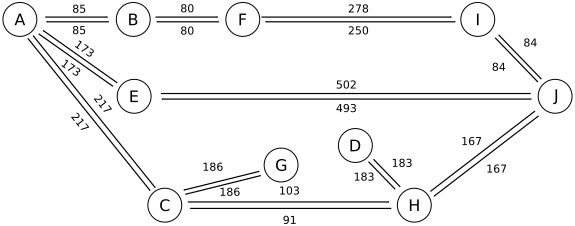
\includegraphics{directed_graph.pdf}
   \caption{\label{directed_graph} Exemple de graphe orienté}
\end{figure}

En théorie des graphes, un graphe orienté est un ensemble de points (ici, des stations) connectés par des flèches (ici, des connexions). Dans le cadre de ce projet, chaque flèche représente une possibilité de relier deux points, dans un sens précis, et avec un coût déterminé. C'est une connection possible entre ces points.

Le problème du plus court chemin, dans ce système, est d'évaluer le coût minimal pour aller d'un point A à un point B. L'algorithme de Dijkstra est une méthode de calcul afin de résoudre ce problème.\\

Cet algorithme peut s'appliquer sur des graphes orientés, modèle auquel plusieurs réseaux de transports sont disponibles (RATP, SNCF, routes, etc), et est également une porte d'entrée pour le domaine de la théorie des graphes, dont certains algorithmes sont vus également dans l'unité d'enseignement [4AI04] Intelligence artificielle.\\

\subsection{Méthode de développement, et outils de la \emph{STL}}

Un programme informatique est une suite d'instructions mathématiques. A ce titre il existe deux difficultés lorsqu'on veut construire un programme informatique pour répondre à un problème :
\begin{enumerate}
\item Quel jeu d'instructions choisir pour répondre au problème algorithmique?\\
La solution ici à été trouvée par l'informaticien Edsger Dijkstra, répondant au problème du plus court chemin énoncée ci-dessus.

\item Comment structurer, implémenter mon problème algorithmique, qui requiert ici la construction de centaines de milliers d'instructions machine, avec la méthodologie nécéssaire pour que n'importe quel humain puisse maintenir ce code et y ajouter des fonctionnalités?\\
Cette question est en partie résolue par l'outil C++. C'est une méthodologie, permettant de générer une grande compléxité dans le jeu d'instructions (comme beaucoup d'outils informatiques), mais également d'utiliser une interface compréhensible, qui vous est donnée ici, et va permettre l'ajout de fonctionnalités de manière concise et ergonomique, en détachant les différentes fonctionnalités, permettant de fournir au final une solution élégante et ré-utilisable.
\end{enumerate}


Afin de résoudre ce problème, des fichiers contenant les points d'un graphe, et contenant des connexions, sont mis à votre disposition. La lecture de ces fichiers devra être réalisée avec des conteneurs spécifiques imposés. Puis, un calcul du chemin le plus court devra être réalisé.\\

Afin de travailler les connaissances vues en cours, nous allons utiliser la \emph{Standard Template Library}, une bibliothèque C++ parmi tant d'autres, mais qui a l'avantage d'être très puissante dans plusieurs modalités, notamment pour les conteneurs que celle-ci propose. Ceux-ci représentent des tableaux associatifs, généralisation des tableaux où les indices ne sont pas forcément des entiers.\\

Une table de hachage est une structure de données efficace pour représenter un tableau associatif, avec une réprésentation mémoire compacte, via le hachage des données qui, dans ce cas, correspond au passage d'un point du graphe par le pointeur vers l'objet correspondant. Les éléments à insérer dans le conteneur ne sont pas forcément triés. Ce sont les raisons pour lesquelles nous utiliseront le conteneur \texttt{std::unordered\_map}, ressemblant (d'un point de vue utilisateur) au conteneur \texttt{std::map} vu en cours, qui implémente lui un arbre binaire de recherche pour garantir l'ordre des données.%les différences citées ci-dessus.

Ces conteneurs vont garder les données du graphe fourni via des fichiers qu'il faudra lire et dont les données doivent être extraites.
Dans ce cas précis, l'utilisation de la bibliothèque standard est fortement conseillé, via la class \texttt{std::ifstream}, prenant en argument le nom du fichier à lire. Une des différentes méthodes pour lire une ligne est d'utiliser la fonction membre \texttt{getline}. On notera que \texttt{std::ifstream}, à l'instar \texttt{std::cin}, possède les propriétés de la class \texttt{std::istream} et donc naturellement une surcharge de l'opérateur de flux entrant.\\

Une auto-évaluation vous est proposée au chapitre \ref{sec::autoeval}, afin de construire progressivement les fonctions nécéssaires à l'accomplissement du projet, et d'ajuster le temps nécéssaire pour le terminer.

\section{Charte d'écriture}
\label{sec::charte}
La startup qui vous a embauché dans ce projet vous impose une charte d'écriture afin de pouvoir maintenir le code et facilitier la transmission au sein de l'équipe.


Celle charte, relativement légère, est énoncée dans un ordre quelconque:
\begin{itemize}
\item \textbf{Utilisation des drapeaux de compilation -Wall -Wextra -Werror -pedantic -pedantic-errors -O3 de g++} afin de garantir le respect de l'implémentation dans les normes C++, et d'optimiser la compilation;
\item \textbf{Utilisation des fonctionnalités du C++ 11 maximum} afin d'utiliser les ressources du cours; %https://msdn.microsoft.com/fr-fr/library/hh567368.aspx
\item \textbf{Proscription de l'utilisation des outils d'allocation dynamique} : \emph{new}, \emph{new[]}, \emph{delete} et \emph{delete[]}, afin d'optimiser la sécurité, la lisibilité, et de tirer parti du concept \emph{RAII} : l'acquisition d'une ressource est une initialisation;
\item \textbf{Mémoire dynamique via les conteneurs de la \emph{STL}} ou les outils de \texttt{memory} comme par exemple \texttt{std::unique\_ptr}, celui-ci étant inutile dans le cadre du projet;
\item \textbf{Indentation parfaite du code source du programme} afin de garantir la lisibilité et de prévenir les erreurs d'implémentation;
\item \textbf{Minimisation de duplication du code source du programme} afin d'éviter le dangereux copier-coller est les graves problèmes de maintenance qui s'y accompagne;
\item \textbf{Obligation d'utilisation de la convention \emph{snake\_case}}, avec des noms de fonctions en \emph{verbe\_complément}, de variables en \emph{complément\_nom}, afin de garantir la lisibilité du code;
\item \textbf{Tout type créé commence par une majuscule}; % kézako
\item \textbf{Les constantes déclarées via \emph{define} sont écrites intégralement en majuscules}; on parlera ici de \emph{SCREAMING\_SNAKE\_CASE};
\item \textbf{Membres de classes appelés via \emph{this}} afin de répèrer facilement l'utilisation et la modification d'outils interne;
\item \textbf{Variables d'entrées précédées d'un underscore \emph{\_}}, pour faciliter la différenciation avec les autres types de variables;
% \item \textbf{Variables locales neutres}; % kézako
\item \textbf{Utilisation du mot clef \emph{const} lorsque l'entrée ne doit pas être modifiée}, afin de garantir ses droits d'accès en lecture/écriture;
\item \textbf{Utilisation systématique de référence ou de pointeur lors du passage d'un objet}, pour des raisons évidentes de passage par référence;
% \item \textbf{Respect du typage lors des comparaisons au moyen de \emph{static\_cast$<$Type$>$(var)} si nécessaire}.
\end{itemize}

\pagebreak

\section{Objectifs}

Un des buts de ce projet est de permettre l'assemblage de code de plus en plus complet, avec un écosystème compréhensible alors qu'il grossit. La méthodologie va montrer cette difficulté, et
c'est pourquoi les objets englobent ces fonctionnalités. \\

Le point le plus important dans le cadre de ce projet est de comprendre l'interface, la structure imposée. Le travail demandé, qui est d'implémenter les fonctionnalités clés, ne sera pas possible sans la compréhension de cette structure. Il est aussi judicieux de se renseigner sur les outils possibles et nécéssaires pour réussir le projet.\\

Les classes doivent hériter d'une classe mère virtuelle pure sans implémentation. Ce principe permet de rajouter des fonctionnalités à une classe sans l'altérer et en garantissant son appel via un pointeur.
Si la classe respecte le contrat, elle garantit d'avoir implémenter les fonctionnalités nécéssaires à la validité du programme. Cela n'empeche pas de pouvoir améliorer et ajouter diverses fonctionnalités supplémentaires, notamment celle proposée en amélioration dans le chapitre suivant. \\

\section{Auto-évaluation}
\label{sec::autoeval}
Parmi les fichiers de l'archive du projet se trouve la classe \texttt{Grade} au travers de \texttt{Grade.hpp} et \texttt{Grade.o}.
En incluant le fichier binaire à la compilation et l'entête au programme principal du projet deux objets static sont automatiquement créés afin de permettre l'évaluation des différentes parties du projet.
Pour rappel, un objet static est un objet alloué au lancement du programme et détruit à sa toute fin (ex: \texttt{std::cout}, \texttt{std::cin}). Il est de plus unique, au sens non rédéfinissable, pour l'ensemble du code à sa portée.
Ces objets se nomme, \texttt{travel::evaluate\_small} et \texttt{travel::evaluate}.
Le premier évaluant le réseau simple, le second évaluant le réseau RATP.
3 méthodes sont à notées:
\begin{itemize}
  \item \texttt{stations(const travel::Generic\_station\_parser\&)}, qui évalue de manière exaustive la construction de la table de stations.
  \item \texttt{connections(const travel::Generic\_connection\_parser\&)}, qui évalue de manière exaustive la construction de la table de connections.
  \item \texttt{dijkstra(travel::Generic\_mapper\&,bool)}, qui évalue dans un premier temps 9 trajets tests, puis propose une exploration exaustive des trajets via une estimation grossière du temps de calcul.
    \begin{itemize}
      \item false: évaluation du projet dans sa version de base (référence de temps de calcul pour le réseau RATP ~324us/trajet, ~6mins de test).
      \item true: évaluation du projet dans sa version de bonus, via l'utilisation de noms de stations au lieu d'id (référence de temps de calcul pour le réseau RATP ~1.5ms/trajet, ~27mins de test).
    \end{itemize}
\end{itemize}
Lorsque une méthode est appelée, elle appelle automatiquement les méthodes précédentes pour garantir le matient des acquis au fur et à mesure de l'avancement du projet.
Il n'est donc pas nécessaire d'appeler les anciens tests.
De plus, il est à noté que la classe de test est indépendante des fichiers de l'archive et apporte toujours une résolution via les fichiers de références du projet.

\section{Feuille de route}
\label{sec::feuille}
L'équipe de développement de votre start-up vous propose une feuille de route, permettant de représenter les diverses tâches et l'avancement du projet :

\begin{enumerate}
\item Instanciez une classe dérivée : faites un nouveau fichier, une inclusion de la classe parente et créez une classe qui hérite de la classe mère \texttt{Generic\_station\_parser}.\\
Le code compile-t-il? Pourquoi?
\item Surchargez la fonction \texttt{read\_stations} : écrivez le prototype de la fonction en ajoutant à la fin le mot clé \texttt{override}, en mettant un corps vide à cette fonction.
Le code compile-t-il? Pourquoi?
\item Ecrivez le corps de la fonction.
\item Créez un fichier avec une fonction principale, instanciez votre classe et appelez la méthode de \texttt{stations} de la classe \texttt{Grade}.\\

\emph{A ce point, vous devriez commencer la deuxième séance de TP}
\item Changer la classe parente pour désomais utiliser la classe de connection (changer l'include aussi), le code compile t'il, pourquoi?
\item Implémentez la/les fonction(s) manquantes.
\item A ce stade, la méthode \texttt{connections} de la class \texttt{Grade} devrait fonctionner.\\

\emph{A ce point, vous devriez commencer la troisième séance de TP}
\item Changer la classe parente pour désomais utiliser la classe de mapper (changer l'include aussi), le code compile t'il, pourquoi?
\item Implémentez la/les fonction(s) manquantes.
\item A ce stage, la méthode \texttt{dijkstra} de la class \texttt{Grade} avec le second argument à \texttt{false} devrait fonctionner.
  %faire les fonctions compute travel, et compute\_and\_display\_travel, avec les arguments en uint64\_t
\item Bonus: implémenter une surcharge de la/les fonction(s) qui estim(ent) le trajet minimal pour assigner les stations de départ et d'arrivée via leurs noms et non plus leurs identifiants.
\item A ce stage, la méthode \texttt{dijkstra} de la class \texttt{Grade} avec le second argument à \texttt{true} devrait fonctionner.
\end{enumerate}

%% \section{Autoévaluation}

%% FIXME : Ici la description des outils d'auto-évaluation

%% RAJOUTER DES TRUCS, snippet de code, appendix de std::machin?

\end{document}
